% --------------------------------------------------------------
% This is all preamble stuff that you don't have to worry about.
% Head down to where it says "Start here"
% --------------------------------------------------------------
 
\documentclass[12pt]{article}
 
\usepackage[nouppercase,headsepline,footsepline,plainfootsepline]{scrpage2}
\automark{section}
\pagestyle{scrheadings}
%\clearscrheadfoot
\ihead{Math 632}
%\ofoot[\pagemark]{\pagemark}% Optional argument controls chapter-starting pages
\ifoot[(Author)]{{\sl \hfill Meenmo K.}}


\usepackage[margin=1in]{geometry} 
\usepackage{amsmath,amsthm,amssymb,scrextend}
\usepackage{fancyhdr}
\usepackage{enumitem}
\usepackage{amsmath}
\usepackage{amssymb}
\usepackage{textcomp}
\usepackage{fancybox}
\usepackage{tikz}
\usepackage{tasks}
\pagestyle{fancy}
\usepackage[makeroom]{cancel}
\usepackage{graphicx}
\usepackage{caption}
\usepackage{mwe}
\usepackage{tikz}
\usetikzlibrary{positioning}

\newcommand{\N}{\mathbb{N}}
\newcommand{\Z}{\mathbb{Z}}
\newcommand{\I}{\mathbb{I}}
\newcommand{\R}{\mathbb{R}}
\newcommand{\Q}{\mathbb{Q}}
\renewcommand{\qed}{\hfill$\blacksquare$}
\let\newproof\proof
\renewenvironment{proof}{\begin{addmargin}[1em]{0em}\begin{newproof}}{\end{newproof}\end{addmargin}\qed}
% \newcommand{\expl}[1]{\text{\hfill[#1]}$}
\setlength{\parindent}{0pt}
\newenvironment{theorem}[2][Theorem]{\begin{trivlist}
\item[\hskip \labelsep {\bfseries #1}\hskip \labelsep {\bfseries #2.}]}{\end{trivlist}}
\newenvironment{lemma}[2][Lemma]{\begin{trivlist}
\item[\hskip \labelsep {\bfseries #1}\hskip \labelsep {\bfseries #2.}]}{\end{trivlist}}
\newenvironment{problem}[2][Problem]{\begin{trivlist}
\item[\hskip \labelsep {\bfseries #1}\hskip \labelsep {\bfseries #2.}]}{\end{trivlist}}
\newenvironment{exercise}[2][Exercise]{\begin{trivlist}
\item[\hskip \labelsep {\bfseries #1}\hskip \labelsep {\bfseries #2.}]}{\end{trivlist}}
\newenvironment{reflection}[2][Reflection]{\begin{trivlist}
\item[\hskip \labelsep {\bfseries #1}\hskip \labelsep {\bfseries #2.}]}{\end{trivlist}}
\newenvironment{proposition}[2][Proposition]{\begin{trivlist}
\item[\hskip \labelsep {\bfseries #1}\hskip \labelsep {\bfseries #2.}]}{\end{trivlist}}
\newenvironment{corollary}[2][Corollary]{\begin{trivlist}
\item[\hskip \labelsep {\bfseries #1}\hskip \labelsep {\bfseries #2.}]}{\end{trivlist}}
 
 
\begin{document}
\begin{section}{\bf Detailed Balance and Reversible Markov Chain}
{\bf Definition} Let $p$ be a transition probability matrix on $S$ and $\mu\colon\; S\to [0,\infty)$ a measure on $S$. Then we say that \underline{detailed balance} holds if $$\mu(x)p(x,y) = \mu(y)p(y,x)\;\;\forall\text{ states } x,y\in S.$$  
when this holds, $\mu$ is a reversible measure for $p$.

\vspace{1\baselineskip}
If $\pi$ is a probability measure $\left(\sum\limits_x \pi(x) = 1\right)$ and $\pi(x)p(x,y)=\pi(y)p(y,x)\;\;\forall\;x,y\in S,$ we call $\pi$ a \underline{reversible distribution} on reversible probability measure.


\begin{enumerate}[label=(\roman*)]
    \item reversible $\to$ stationary
    $$\sum\limits_x \mu(x)p(x,y) = \sum\limits_x \mu(y)p(y,x)=\mu(y)\sum\limits_x p(y,x)=\mu(y)$$\\
    
    {\bf Example} 2-State Chain
    $$p=\begin{pmatrix}
    1-a&a\\b&1-b
    \end{pmatrix}
    \qquad
    \text{ Invariant: }\pi = \begin{pmatrix}
    \frac{b}{a+b}&\frac{a}{a+b}
    \end{pmatrix}$$
    Check Detailed Balance
    $$\pi(1)\cdot p(1,2)=\pi(2)\cdot p(2,1)\qquad
    \frac{b}{a+b}\cdot a = \frac{a}{a+b}\cdot b$$
    
    \item Success Runs
    
    
$$
    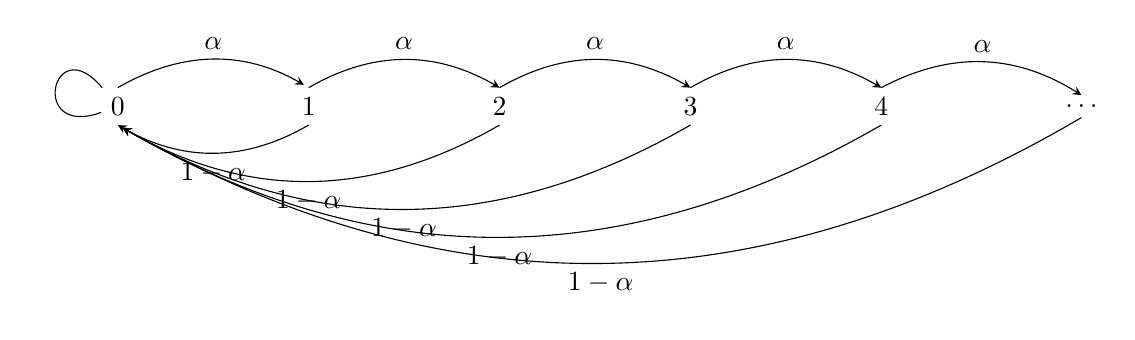
\begin{tikzpicture}
      \node (a) {0};
      \node[right=2cm of a] (b) {1};
      \node[right=2cm of b] (c) {2};
      \node[right=2cm of c] (d) {3};
      \node[right=2cm of d] (e) {4};
      \node[right=2cm of e] (f) {$\ldots$};
    
      \draw (a) to [out=130,in=200,looseness=8] (a);
      %a>b
      \draw[-stealth,shorten >= 2pt] (a.north) to[bend left] node[midway,above] {$\alpha$} (b.north);
      \draw[-stealth] (b.north) to[bend left] node[midway,above] {$\alpha$} (c.north);
      \draw[-stealth] (c.north) to[bend left] node[midway,above] {$\alpha$} (d.north);
      \draw[-stealth] (d.north) to[bend left] node[midway,above] {$\alpha$} (e.north);
      \draw[-stealth] (e.north) to[bend left] node[midway,above] {$\alpha$} (f.north);
    
      %b>a
      \draw[-stealth] (b.south) to[bend left] node[midway,below] {$1-\alpha$} (a.south);
      \draw[-stealth,shorten >= 2pt] (d.south) to[bend left] node[midway,below] {$1-\alpha$} (a.south);
      \draw[-stealth,shorten >= 2pt] (e.south) to[bend left] node[midway,below] {$1-\alpha$} (a.south);
      \draw[-stealth,shorten >= 2pt] (f.south) to[bend left] node[midway,below] {$1-\alpha$} (a.south);
      \draw[-stealth,shorten >= 2pt] (c.south) to[bend left] node[midway,below] {$1-\alpha$} (a.south);
    \end{tikzpicture}
    $$
    $$\pi(2)_{>0}\cdot p(2,3)_{>0} = \pi(3)_{>0}\cdot p(3,2)_{=0} \qquad \qquad\text{Doesn't hold Detailed Balance}$$
    
    \newpage
    \item Reflected Random Walk
    $$
            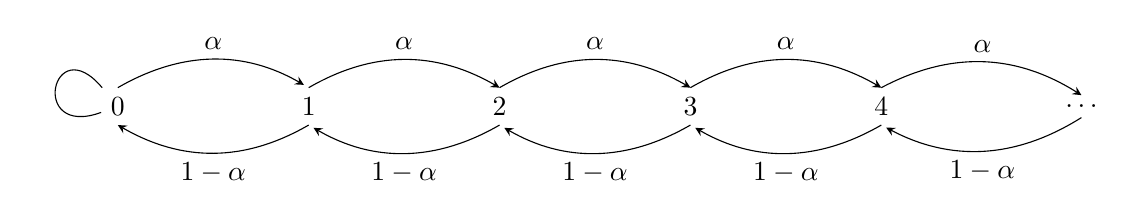
\begin{tikzpicture}
              \node (a) {0};
              \node[right=2cm of a] (b) {1};
              \node[right=2cm of b] (c) {2};
              \node[right=2cm of c] (d) {3};
              \node[right=2cm of d] (e) {4};
              \node[right=2cm of e] (f) {$\ldots$};
            
              \draw (a) to [out=130,in=200,looseness=8] (a);
              %a>b
              \draw[-stealth,shorten >= 2pt] (a.north) to[bend left] node[midway,above] {$\alpha$} (b.north);
              
              %b>c
              \draw[-stealth] (b.north) to[bend left] node[midway,above] {$\alpha$} (c.north);
              \draw[-stealth] (c.north) to[bend left] node[midway,above] {$\alpha$} (d.north);
              \draw[-stealth] (d.north) to[bend left] node[midway,above] {$\alpha$} (e.north);
              \draw[-stealth] (e.north) to[bend left] node[midway,above] {$\alpha$} (f.north);
            
              %b>a
              \draw[-stealth] (b.south) to[bend left] node[midway,below] {$1-\alpha$} (a.south);
              
              %c>b
              \draw[-stealth,shorten >= 2pt] (d.south) to[bend left] node[midway,below] {$1-\alpha$} (c.south);
              \draw[-stealth,shorten >= 2pt] (e.south) to[bend left] node[midway,below] {$1-\alpha$} (d.south);
              \draw[-stealth,shorten >= 2pt] (f.south) to[bend left] node[midway,below] {$1-\alpha$} (e.south);
              \draw[-stealth,shorten >= 2pt] (c.south) to[bend left] node[midway,below] {$1-\alpha$} (b.south);
            \end{tikzpicture}
            $$
    
    For $0<\alpha<\frac{1}{2}$, the invariant distribution is
    $$\pi(k)=\left(1-\frac{\alpha}{1-\alpha}\right)\left(\frac{\alpha}{1-\alpha}\right)^k$$
    
    Check Detailed Balance:
    $$\pi(k)\cdot p(k,\;k+1) = \pi(k+1)\cdot p(k+1,\;k)$$
    $$\cancel{\left(1-\frac{\alpha}{1-\alpha}\right)}\left(\frac{\alpha}{1-\alpha}\right)^k\cdot \alpha =
    \cancel{\left(1-\frac{\alpha}{1-\alpha}\right)}\left(\frac{\alpha}{1-\alpha}\right)^{k+1}\cdot (1-\alpha)$$
    $$\left(\frac{\alpha}{1-\alpha}\right)^k\cdot \alpha = \left(\frac{\alpha}{1-\alpha}\right)^{k}\cdot\frac{\alpha}{\cancel{1-\alpha}}\cdot \cancel{(1-\alpha)} = \left(\frac{\alpha}{1-\alpha}\right)^k\cdot \alpha $$
\end{enumerate}


\vspace{2\baselineskip}
{\sl Remark.} 
$$P_\mu(X_0=x_0,\ldots,X_n=x_n)=\mu(X_0)\cdot P(X_0,\;X_1)\ldots P(X_{n-1},\;X_n)$$
$$=P\pi(X_n=x,\;X_{n+1}=y) = \pi(x)\cdot p(x,y)$$
$$=P_\pi(X_m=x_0,\ldots,\; X_{m+n}=x_n) = \sum\limits_x \pi(x)p^m(x_0,\;x_1)\ldots p(x_{n-1},x_n)$$

\vspace{1\baselineskip}
{\bf Theorem} Suppose $\pi$ is a reversible distribution, then
$$P_\pi[X_0=x_0,\; X_1=x_1,\ldots , X_n=x_n] = P_\pi[X_0=x_n,\; X_1=x_{n-1},\ldots, X_n=x_0]$$
\end{section}

Come back this part later.

\newpage
V.. the distribution between detailed balance and invariance.
\begin{enumerate}[label=(\roman*)]
    \item Suppose $\pi$ is invariant\\
    [image]
    Gxx each state $x$ an invariant $\pi(x)$ of "mass.\\
    
    Let the mass flow along the edge: state $x$ sends amount $\pi(x)p(x,y)$ to each state $y$.\\
    [image]
    
    \vspace{1\baselineskip}
    How much mass does $y$ have after the completion of flows?
    $$\sum\limits_x \pi(x)\cdot p(x,y)=\pi(y)\to\text{ Some mass distribution as before}$$
    
    \item suppose $\pi$ is reversible: $\pi(x)\cdot p(x,y) = p(y)\pi(y,x)$\\
    [image]
    
    \vspace{1\baselineskip}
    Flows from $x$ to $y$ and $y$ to $x$ balance out between all pairs of states ($\pi=\pi p)$.
    
    \item Random walk on an undirected graph ("network"): $G=(V,E)$ where $V$: Vertices and $E$: Edges between vertices.[image]
    
    \item Adjacency Matrix: $A=(a(u,v))\to$ symmetric [image]
    $$a(u,v)=\begin{cases}1\qquad \text{if } <u,v>\in E\\
    0\qquad \text{if } <u,v> \notin E
    \end{cases}$$
    $$A=\begin{pmatrix}
    1&0&1&0\\0&0&1&1\\1&1&0&1\\0&1&1&1
    \end{pmatrix}$$
    
    Degree of a vertex: $d(u)$: the number of edges attached to it.\\
    
    Random walk on a graph: $X_n$ jumps from its current location by choosing unifromly at random one of the edges available to it.\\
    
    Transition probability: 
    $$p(u,v)=\begin{cases}
    \frac{a(u,v)}{d(u)}\\ 1\qquad\text{if $u=v$ and $d(u)=0$}
    \end{cases}$$
    Come back later.
\end{enumerate}

\newpage
[image]

\vspace{1\baselineskip}
Suppose that $x\in T$ ($x$ is transient). There will be a first time when we visit $R$.
$$\begin{cases}
\text{Exist distribution}\qquad P(A) = \sum P(A|B)P(B)\\
\text{Exit time}\qquad E(Y)= \sum\limits_i E(Y|B_i)P(B_i)
\end{cases}
$$
\end{document}